\section{Introduction}

Recent advances in offline reinforcement learning (RL) make it possible to train policies for real-world scenarios, such as robotics~\citep{kalashnikov2018scalable,Rafailov2020LOMPO, kalashnikov2021mt} and healthcare~\citep{guez2008adaptive,shortreed2011informing,killian2020empirical}, entirely from previously collected data. Many realistic settings where we might want to apply offline RL are inherently \emph{multi-task} problems, where we want to solve multiple tasks using all of the data available. For example, if our goal is to enable robots to acquire a range of different behaviors, it is more practical to collect a modest amount of data for each desired behavior, resulting in a large but heterogeneous dataset, rather than requiring a large dataset for every individual skill. Indeed, many existing datasets in robotics~\citep{finn2017deep,dasari2020robonet,sharma2018multiple} and offline RL~\citep{fu2020d4rl} include data collected in precisely this way. Unfortunately, leveraging such heterogeneous datasets leaves us with two unenviable choices. We could train each task only on data collected for that task, but such small datasets may be inadequate for good performance. Alternatively, we could combine all of the data together \arxiv{and use data relabeled from other tasks to improve offline training}, but this na\"{i}ve data sharing approach can actually often degrade performance over simple single-task training in practice~\citep{kalashnikov2021mt}. 
In this paper, we aim to understand how data sharing affects RL performance in the offline setting and develop a reliable and effective method for selectively sharing data across tasks.

A number of prior works have studied multi-task RL in the \emph{online} setting, confirming that multi-tasking can often lead to performance that is worse than training tasks individually~\cite{parisotto2015actor,rusu2015policy,yu2020metaworld}. These prior works focus on mitigating optimization challenges that are aggravated by the online data generation process~\cite{schaul2019ray,yu2020gradient,yang2020multi}. As we will find in Section~\ref{sec:analysis}, multi-task RL remains a challenging problem in the offline setting when sharing data across tasks, even when exploration is not an issue. While prior works have developed heuristic methods for reweighting and relabeling data~\citep{andrychowicz2017hindsight,eysenbach2020rewriting, li2020generalized,kalashnikov2021mt}, they do not yet provide a principled explanation for why data sharing can hurt performance in the offline setting, nor do they provide a robust and general approach for selective data sharing that alleviates these issues while preserving the efficiency benefits of sharing experience across tasks.

In this paper, we hypothesize that data sharing can be harmful or brittle in the offline setting because it can exacerbate the distribution shift between the policy represented in the data and the policy being learned. 
We analyze the effect of data sharing in the offline multi-task RL setting, and present evidence to support this hypothesis.
Based on this analysis, we then propose an approach for selective data sharing that aims to minimize distributional shift, by sharing only data that is particularly relevant to each task. Instantiating a method based on this principle requires some care, since we do not know a priori which data is most relevant for a given task before we've learned a good policy for that task.
\arxiv{To provide a practical instantiation, we propose the conservative data sharing (CDS) algorithm. CDS reduces distributional shift by sharing data based on a learned conservative estimate of the Q-values that penalizes Q-values on out-of-distribution actions. Specifically, CDS relabels transitions when the conservative Q-value of the added transitions exceeds the expected conservative Q-values on the target task data. We visualize how \cdsmethodname\ works in Figure~\ref{fig:teaser}.}

\begin{wrapfigure}{r}{7cm}
    \vspace{-0.3cm}
    \centering
    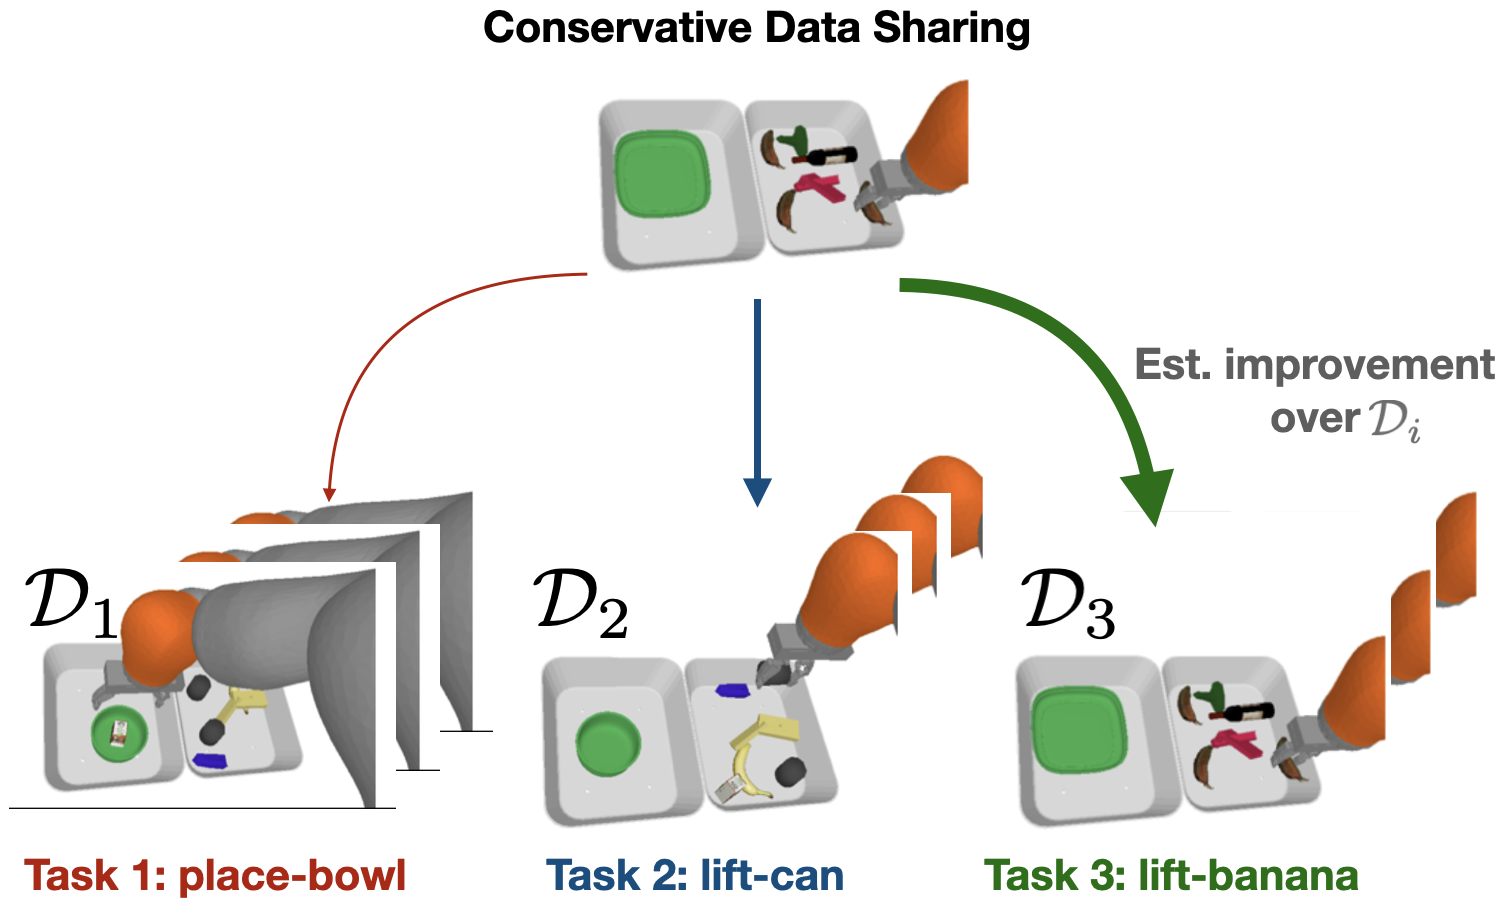
\includegraphics[width=0.45\textwidth]{chapters/cds/cds_teaser.png}
    %%SL.7.31: consider making this a wrapfigure
    \vspace{-0.2cm}
    \caption{\footnotesize A visualization of \cdsmethodname, which routes a transition to
    the offline dataset $\mathcal{D}_i$ for each task $i$ with a weight based on the estimated improvement over the behavior policy $\pi_\beta(\ba|\bs, i)$ of $\mathcal{D}_i$ after sharing the transition.}
    \label{fig:teaser}
    \vspace{-0.3cm}
\end{wrapfigure}


The main contributions of this work are an analysis of data sharing in offline multi-task RL and a new algorithm, \textit{conservative data sharing} (\cdsmethodname), for multi-task offline RL problems. \arxiv{\cdsmethodname\ relabels a transition into a given task only when it is expected to improve performance based on a conservative estimate of the Q-function.} 
After data sharing, similarly to prior offline RL methods, \cdsmethodname\ applies a standard conservative offline RL algorithm, such as CQL~\citep{kumar2020conservative}, that learns a conservative value function or BRAC~\citep{wu2019behavior}, a policy-constraint offline RL algorithm. Further, we theoretically analyze \cdsmethodname\ and characterize scenarios under which it provides safe policy improvement guarantees. Finally, we conduct extensive empirical analysis of \cdsmethodname\ on multi-task locomotion, multi-task robotic manipulation with sparse rewards, multi-task navigation, and multi-task imaged-based robotic manipulation. We compare CDS to vanilla offline multi-task RL without sharing data, to na\"{i}vely sharing data for all tasks, and to existing data relabeling schemes for multi-task RL. \cdsmethodname\ is the only method to attain good performance across all of these benchmarks, often significantly outperforming the best \textit{domain-specific} method, improving over the next best method on each domain by \textbf{17.5\%} on average.